
\section{Syntactic arguments}\label{syntactic-sec}

Many proofs or refutations of implications (or equivalences) between two equational laws $E,E'$ can be obtained from the syntactic form of the equation.  We discuss some techniques here that were useful in the ETP.

\subsection{Simple rewrites}\label{rewrite-sec}

Many equational laws $E'$ can be formally deduced from a given law $E$ by applying the \emph{Lean} \texttt{rw} tactic to rewrite $E'$ repeatedly by some forward or backward application of $E$ applied to arguments that match some portion of $E$.  For instance, the commutative law \eqref{eq43} clearly implies $\x \op (\y \op \z) \formaleq (\y \op \z) \op \x$ \eqref{eq4531}
by a single such rewrite.  A brute force application of such rewrite methods is already able to directly generate about $\num{15000}$ such implications, including many equivalences to the singleton law \eqref{eq2} and the constant law \eqref{eq46}.  After applying transitive closure, this generates about four million further such implications.

A simple observation that already generates a reasonable number of equivalences is that any equation of the form $\x \formaleq f(\y,\z,\dots)$ necessarily is equivalent to the trivial law $\x \formaleq \y$, by transitivity; similarly, an equation of the form $f(\x,\y) \formaleq g(\z,\w,\dots)$ implies $f(\x,\y) \formaleq f(\x',\y')$; and so forth.  Equivalences of this form were useful early in the project by cutting down the number of distinct equivalence classes of laws that needed to be studied.

\subsection{Matching invariants}

Fix an alphabet $X$. A \emph{matching invariant} is an assignment $I \colon \Magma_X \to {\mathcal I}$ of an object $I(w) \in {\mathcal I}$ in some space ${\mathcal I}$ to each word $w \in \Magma_X$ with the property that if an equational law $w_1 \formaleq w_2$ has matching invariants $I(w_1)=I(w_2)$, then the same matching $I(w'_1) = I(w'_2)$ holds for any consequence $w'_1 \formaleq w'_2$.  In particular, if one law $I(w_1)=I(w_2)$ and $I(w'_1) \neq I(w'_2)$, then the law $w_1 \formaleq w_2$ does not imply the law $w'_1 \formaleq w'_2$.

A simple example of a matching invariant is the multiplicity $(n_x)_{x \in X}$ of variables of a word: if $w_1,w_2$ have all variables $x$ appear the same number of times $n_x$ in both words, then any rewriting of a word $w$ using the law $w_1 \formaleq w_2$ will preserve this property.  Hence, if $w'_1, w'_2$ do not have that each variable appear the same number of times in both words, then $w_1 \formaleq w_2$ cannot imply $w'_1 \formaleq w'_2$.  For instance, the commutative law \eqref{eq43} cannot imply the left-absorptive law \eqref{eq4}.

One source of matching invariants comes from the free magma $\Magma_{X,\Gamma}$ of a theory:

\begin{proposition}[Free magmas and matching invariants]\label{free-inv}  Let $\iota_{X,\Gamma} \colon X \to \Magma_{X,\Gamma}$ be the map associated to the free magma $\Magma_{X,\Gamma}$ for a theory $\Gamma$.  Then the map $I \colon \Magma_X \to \Magma_{X,\Gamma}$ defined by $I(w) \coloneqq \varphi_{\iota_{X,\Gamma}}(w)$ is an invariant.
\end{proposition}

\begin{proof}  Suppose that $w_1 \formaleq w_2$ entails $w'_1 \formaleq w'_2$, and that $I(w_1) = I(w_2)$.  For any $f \colon X \to \Magma_{X,\Gamma}$, the two maps $\varphi_f, \varphi_{f,\Gamma} \circ \varphi_{\iota_{X,\Gamma}} \colon \Magma_X \to \Magma_{X,\Gamma}$ are both homomorphisms that extend $f$, hence agree by the universal property of $\Magma_X$, as displayed by the following commutative diagram:
\[\begin{tikzcd}
	&& X \\
	\\
	{\Magma_X} && {\Magma_{X,\Gamma}} && {\Magma_{X,\Gamma}}
	\arrow[hook, from=1-3, to=3-1]
	\arrow["{\iota_{X,\Gamma}}", pos=0.7, left, from=1-3, to=3-3]
	\arrow["f", pos=0.7, above, from=1-3, to=3-5]
	\arrow["{I = \varphi_{\iota_{X,\Gamma}}}", pos=0.6, above, from=3-1, to=3-3]
	\arrow["{\varphi_f}"', curve={height=18pt}, pos=0.6, below, from=3-1, to=3-5]
	\arrow["{\varphi_{f,\Gamma}}", pos=0.5, above, from=3-3, to=3-5]
\end{tikzcd}\]
In particular, the hypothesis $I(w_1)=I(w_2)$ implies that $\varphi_f(w_1) = \varphi_f(w_2)$ for all $f \colon X \to \Magma_{X,\Gamma}$; that is to say, the magma $\Magma_{X,\Gamma}$ obeys the law $w_1 \formaleq w_2$, and hence also $w'_1 \formaleq w'_2$ by hypothesis.  Thus $\varphi_{\iota_{X,\Gamma}}(w'_1) = \varphi_{\iota_{X,\Gamma}}(w'_2)$, which gives $I(w'_1) = I(w'_2)$ as required.
\end{proof}

\begin{example}  If we take $\Gamma = \{\Eq{4}\}$ to be the theory of the left-absorptive law \eqref{eq4} as described in \Cref{left-absorb}, then the matching invariant $I(w)$ produced by \Cref{free-inv} is the left-most letter of the alphabet $X$ appearing in the word; for instance $I((\x \op \y) \op \z) = \x$.  Thus, for example, the left-absorptive law \eqref{eq4} cannot imply the right-absorptive law \eqref{eq5}.
\end{example}

\begin{example}  If we take $\Gamma = \{\Eq{43}, \Eq{4512}\}$ to be the theory of the commutative law \eqref{eq43} and the associative law \eqref{eq4512}, then by \Cref{semi-group}, the associated invariant $I(w) = \sum_{x \in X} n_x e_x$ is the formal sum of all the generators $e_x$ appearing in the word $w$, in the free abelian semigroup generated by those generators.  This recovers the preceding observation that the multiplicities $(n_x)_{x \in X}$ form a matching invariant.
\end{example}

\begin{example}  Let $n \geq 1$ be a positive integer, and consider the theory $\Gamma = \{\Eq{43}, \Eq{4512}, E_n\}$ consisting of the previous theory $\{\Eq{43}, \Eq{4512}\}$ together with the order-$n$ law $L_x^y x = y$.  One can check that the free magma $\Magma_{X,\Gamma}$ can be described as the free group of exponent $n$ with generators $e_x, x \in X$, with associated map $\iota_{X,\Gamma} \colon x \mapsto e_x$.  The associated matching invariant $I(w) = \sum_{x \in X} n_x e_x$ is essentially the multiplicities $(n_x \hbox{ mod } n)_{x \in X}$ modulo $n$, which gives a slightly stronger criterion than the preceding matching invariant for refuting implications.  For example, the cubic idempotent law $\x \formaleq (\x \op x) \op \x$ \eqref{eq23}
has matching invariants $e_x = 3e_x$ in the $n=2$ case, and hence does not imply the idempotent law $\x \formaleq \x \op \x$ \eqref{eq3} since $e_x \neq 2e_x$ in the $n=2$ case.
\end{example}

In practice, we found that these invariants could be used to establish a significant fraction of the non-implications in the implication graph, although in most cases these non-implications could also be established by other means, for instance through consideration of small finite counterexamples.

\begin{remark}  One can also obtain matching invariants from the free objects associated to theories that involve additional operations beyond the magma operation $\op$, such as an identity element or an inverse operation.  We leave the precise generalization of \Cref{free-inv} to such theories to the interested reader.
\end{remark}

\subsection{Canonization}\label{canon-sec}

One possible way of obtaining refutations of a given implication $E_1 \Rightarrow E_2$ between equational laws is by building a special kind of syntactic model, via certain involutions on elements of the free magma $\Magma_X$ we call \emph{canonizers}.

\begin{definition}
  A function $C:\Magma_X\rightarrow\Magma_X$ is a \emph{canonizer} for an equation $E$ if
  \begin{enumerate}
    \item $C$ is computable.
    \item if $w_1\sim_E w_2$, then $C(w_1) = C(w_2)$.
  \end{enumerate}
\end{definition}

In fact, a canonizer is simply a matching invariant with target in $\Magma_X$.

We describe a concrete strategy for building such $C$s, which will require a number of definitions.

Let $R$ be an arbitrary function $\Magma_X\rightarrow \Magma_X$.

\begin{definition}\label{def:canon}
  We say that $R$ is (weakly) \emph{collapsing} if for every word $w$, $R(w)$ is a sub-word of $w$ (in the obvious sense).

  A function $\theta : X\rightarrow\Magma_X$ is called a \emph{substitution}, and we can extend $\theta$ to be a homomorphism in the obvious way. We write $w\theta$ instead of $\theta(w)$ for application of substitutions.

  If $E$ is the equation $l\simeq r$, and $l$ is not a variable, we say that $R$ is a \emph{weak canonizer} if for any substitution $\theta$, $R(l\theta)=r\theta$.

  Finally we say that $R$ is \emph{non-overlapping} for $E$ if for every word $w\in\Magma_X$ which is a strict sub-word of $l$ that is not in $X$, and any substitution $\theta$, $R(w\theta) = w\theta$.
\end{definition}

We can then define $C_R : \Magma_X\rightarrow\Magma_X$ as follows:

\begin{align}
  C_R(x) &= x\\
  C_R(w\op w') &= R(C_R(w)\op C_R(w'))
\end{align}

And the following theorem holds.
\begin{theorem}\label{thm:canon}
  Whenever $R$ satisfies all the conditions of Definition \ref{def:canon} then $C_R$ is a canonizer.
\end{theorem}
\begin{proof}
  Assume $w\sim_{E}w'$. We proceed by induction over the proof of equality.

  The only non trivial case is $w = l\theta$ and $w'=r\theta$ for some substitution $\theta$.
  Then we have
  \begin{align}
    C_R(l\theta) &= R(l(C_R\circ\theta)) \\
                 &= r(C_R\circ\theta)\\
                 &= C_R(r\theta)
  \end{align}
  where the first and third equalities follow from non-overlapping and weak collapsing, and the second from weak canonicity.
\end{proof}

We work through an example to show why this is a useful theorem. Take $E$ to be the equation
\[
  y \op (x \op (y \op (y \op y)))\simeq x
\]
we can take $R$ to be the transformation which sends a term of the form $w \op (v \op (w \op (w \op w)))$ to $v$ for any two words $v, w$, and leaves all other words unchanged.
It is then somewhat easy to show that this transformation satisfies the conditions of theorem \ref{thm:canon}, and so we have a canonizer $C_R$.
This can be used, e.g. to refute the implication of $x = (x \op x) \op (x \op (x \op x))$ from the above equality.

As a conclusion for this section, we note that a very general strategy for building canonizers comes from the theory of \emph{rewrite systems}, see e.g. Baader \& Nipkow \cite{term-rewriting}.
In that setting one defines rewriting as a transformation on words (or terms), and if this transformation is \emph{terminating} and \emph{confluent} (intuitively, rewrites cannot go on forever, or diverge forever), then one may simply pick the transformation which sends a term to its normal form as a canonizer.

Though we note that the non-overlapping criterion seems very similar to the notion of orthogonality in rewriting, we leave the investigation of the precise relationship of the classical theory with the above technique as future work.

\subsection{Unique factorization}

In general, the free magma $\Magma_{X,E}$ for a given equational law $E$, which we can canonically define as $\Magma_X/\!\sim_E$, is hard to describe explicitly; indeed, from the undecidability of implications between equational laws, such a magma cannot be computably described for arbitrary $E$.  Nevertheless, for some laws it is possible to obtain some partial understanding of $\Magma_{X,E}$ from a syntactic perspective.  For instance, if we can refute the equivalence $w'_1 \sim_E w'_2$ by constructing a counterexample magma $M$ that obeys $E$ but not $w'_1 \formaleq w'_2$, then this implies that the representatives $\iota_{X,E}(w'_1), \iota_{X,E}(w'_2)$ of  $w'_1, w'_2$ in $\Magma_{X,E}$ are distinct.

We illustrate this approach with equations $E$ of the left-absorptive form
\begin{equation}\label{left-absorptive}
\x \formaleq \x \op f(\x,\y,\z)
\end{equation}
for some word $f(\x,\y,\z)$, that are also known to imply the right-idempotent law \eqref{eq378}.  An illustrative example is the law \eqref{eq854} depicted in Figure \ref{fig:854}. Other examples are listed in \Cref{fig:854-like}.

\begin{figure}
  \centering
  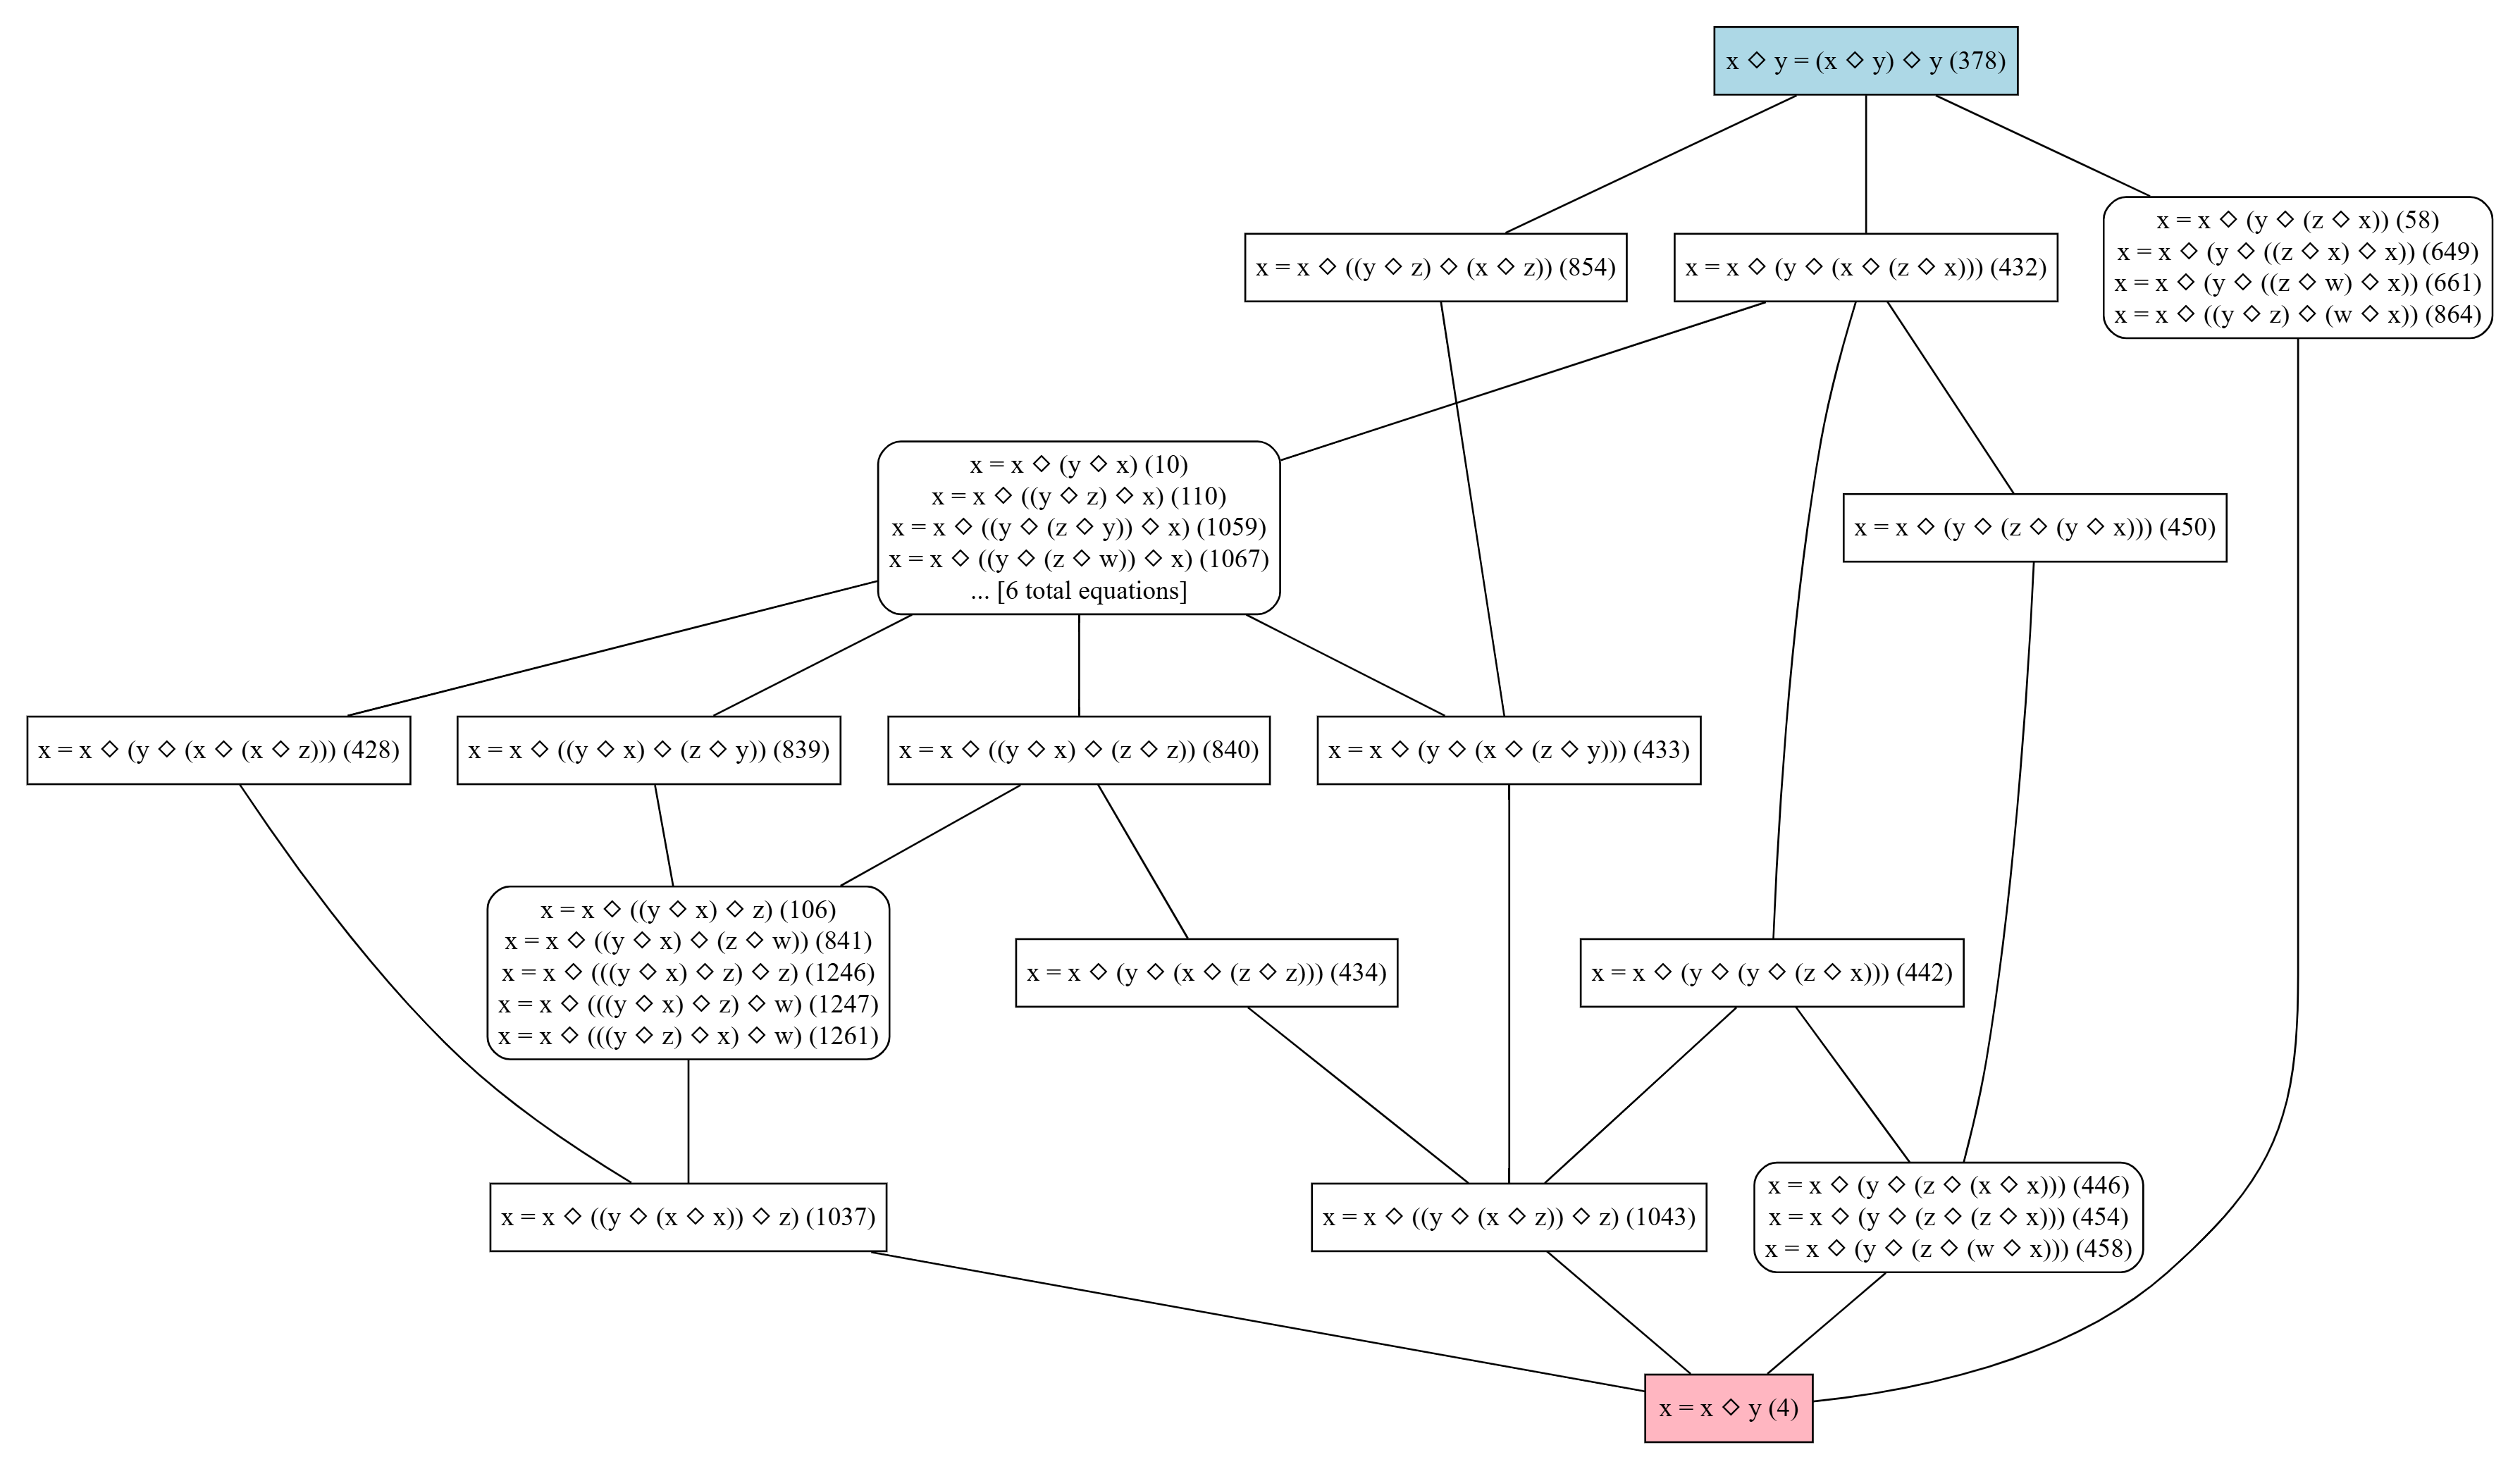
\includegraphics[width=0.85\textwidth]{854-like.png}
  \caption{Equations similar to \eqref{eq854} that are of the form \Cref{left-absorptive} (possibly involving a fourth indeterminate $\w$) and imply \eqref{eq378}.  For brevity, $70$ equations equivalent to \eqref{eq4} have been omitted.}
  \label{fig:854-like}
  \end{figure}


\begin{lemma}\label{854} Equation \eqref{eq854} is of the form \eqref{left-absorptive} and implies \eqref{eq378}.
\end{lemma}

\begin{proof}  Clearly we have \eqref{left-absorptive} with $f(\x,\y,\z) \coloneqq (\y \op \z) \op (\x \op \z)$.  From \ref{left-absorptive} we have in any magma obeying \eqref{eq854} that
$$x = x \op f(x,x,S^2 x) = x \op S(x \op S^2 x) = x \op S(x \op f(x,x,x)) = x \op Sx.$$
This implies from a further application of \Cref{left-absorptive} that
$$ y = y \op f(y,x,y) = (y \op Sy) \op ((x \op y) \op Sy) = f(x \op y, y, Sy)$$
and hence by \Cref{left-absorptive} again
$$ (x \op y) \op y = x \op y$$
giving \eqref{eq378}.
\end{proof}

Let $E$ be a law of the form \eqref{left-absorptive} that implies \eqref{eq378}. We define a directed graph $\to_E$ on words in $\Magma_X$ by declaring $w' \to_E w$ if $w \sim_E w'' \op w'$ for some $w' \in \Magma_X$.  By \eqref{eq378} (applied to the quotient magma $\Magma_{X,E} = \Magma_X/\sim_E$), this is equivalent to requiring that $w \sim_E w \op w'$. In particular, from \eqref{left-absorptive} we have $f(x,y,z) \to x$ for all $x,y,z$.  Furthermore, the relation $\to_E$ factors through $\sim_E$: if $w \sim_E \tilde w$ and $w' \sim_E \tilde w'$, then $w' \to_E w$ if and only if $\tilde w \to_E \tilde w$.

Call a word $w \in \Magma_X$ \emph{irreducible} if it is not of the form $w = w_1 \op w_2$ with $w_2 \to_E w_1$.  We can partially understand the equivalence relation $\sim_E$ on irreducible words:

\begin{theorem}[Description of equivalence]\label{irred-desc}  Let $E$ be an equation of the form \eqref{left-absorptive}.  Let $w$ be an irreducible word, and let $w'$ be a word with $w \sim_E w'$.
  \begin{itemize}
    \item[(i)] If $w$ is a product $w = w_1 \op w_2$, then $w'$ takes the form
$$ w' = (((w'_1 \op w'_2) \op v_1) \op \dots \op v_n)$$
for some $w'_1 \sim_E w_1$, $w'_2 \sim_E w_2$, some $n \geq 0$, and some words $v_1, \dots, v_n$ such that for all $0 \leq i < n$, $v_{i+1}$ is of the form
$$ v_{i+1} \sim_E f(x_i,y_i,z_i)$$
for some $x_i, y_i, z_i$ with
$$ x_i \sim_E (((w'_1 \op w'_2) \op v_1) \op \dots \op v_i).$$
In particular, $v_{i+1} \to_E x_i$.
  \item[(ii)] Similarly, if $w \in X$ is a generator of $\Magma_X$, then $w'$ takes the form
$$ w' = ((w \op v_1) \op \dots \op v_n)$$
for some $n \geq 0$, and some words $v_1, \dots, v_n$ such that for all $0 \leq i < n$, $v_{i+1}$ is of the form
$$ v_{i+1} \sim_E f(x_i,y_i,z_i)$$
for some $x_i, y_i, z_i$ with
$$ x_i \sim_E ((w \op v_1) \op \dots \op v_i).$$
In particular, $v_{i+1} \to_E x_i$.
\end{itemize}
Conversely, any word of the above forms is equivalent to $w$.
\end{theorem}

\begin{proof}  We just verify claim (i), as claim (ii) is similar.  The converse direction is clear from \eqref{left-absorptive} (after quotienting by $\sim_E$), so it suffices to prove the forward claim. By the Birkhoff completeness theorem, it suffices to prove that the class of words described by (i) is preserved by any term rewriting operation, in which a term in the word is replaced by an equivalent term using \eqref{left-absorptive}.  Clearly the term being rewritten is in $w'_1$ or $w'_2$ then the form of the word is preserved, and similarly if the term being rewritten is in one of the $v_i$.  The only remaining case is if we are rewriting a term of the form
$$ x_i = (((w'_1 \op w'_2) \op v_1) \op \dots \op v_i).$$
If $i>0$ we can rewrite this term down to $x_{i-1}$, and this still preserves the required form (decrementing $n$ by one).  If $i=0$ then we cannot perform such a rewriting because of the irreducibility of $w_1 \op w_2$ and hence $w'_1 \op w'_2$.  Finally, we can rewrite $x_i$ to $x_i \op v$ where $v$ is of the form
$$ v_i = f(x_i,y,z),$$
and after some relabeling we are again of the required form (now incrementing $n$ by one). This covers all possible term rewriting operations, giving the claim.
\end{proof}

Specializing to the case where $w,w'$ are both irreducible, we conclude

\begin{corollary}[Unique factorization]\label{unique-factorization}  Two irreducible words $w, w'$ are equivalent if and only if they are either the same generator of $X$, or are of the form $w = w_1 \op w_2$, $w' = w'_1 \op w'_2$ with $w_1 \sim_E w'_1$ and $w_2 \sim_E w'_2$.
\end{corollary}

As an application of this corollary, we establish

\begin{proposition}[$\Eq{854}$ does not imply $\Eq{3316}$]\label{854-3316} Equation \eqref{eq854} does not imply \eqref{eq3316}.
\end{proposition}

\begin{proof}(Sketch)
  We work in the free magma $\Magma_X$ on two generators $X = \{\x,\y\}$.  It suffices to show that
$$  \x \op \y \not \sim_{E854} \x \op (\y \op (\x \op \y)).$$
Suppose this were not the case, then by \Cref{unique-factorization} one of the following statements must hold:
\begin{itemize}
\item[(i)] $y \to_{E854} x$.
\item[(ii)] $(y \op (x \op y)) \to_{E854} x$.
\item[(iii)] $y \op (x \op y) \sim_{E854} y$.
\end{itemize}
If (i) holds, then we have $x \op y = x$ must hold in $\Magma_X/\sim_E$, hence \eqref{eq854} would imply \eqref{eq4}.  However, it is possible to refute this implication by a finite counterexample.

Similarly, if (iii) held, then \eqref{eq854} would have to imply \eqref{eq10}, but this can also be refuted by a finite magma.

Finally, if (ii) held, then the claim
$$  x \op y \sim x \op (y \op (x \op y))$$
to refute simplifies to
$$  x \op y \sim x$$
and we are back to (i), which we already know not to be the case.
\end{proof}
